%-----------------------------------------------------------------------
% Functional Programming 4
% John O'Donnell, Wim Vanderbauwhede
% University of Glasgow
%-----------------------------------------------------------------------

\documentclass{beamer}
\usepackage{jtodlecseriesFP4}
%include polycode.fmt
%format alpha = "\alpha"
%format -- > = "\leadsto "

% Identify this presentation
\SetPresentationTitle
  {Strictness}
  {Strictness}
\SetPresentationNumber
  {9}
\SetPresentationDate
  {Week 5-1}
  {Week 5-1}

%-----------------------------------------------------------------------
% Beginning

\begin{document}

\begin{frame}[fragile]
  \PresentationTitleSlide
\end{frame}

\begin{frame}[fragile]
  \frametitle{Topics}
  \tableofcontents
\end{frame}
%-----------------------------------------------------------------------
\begin{frame}[fragile]
\begin{center}
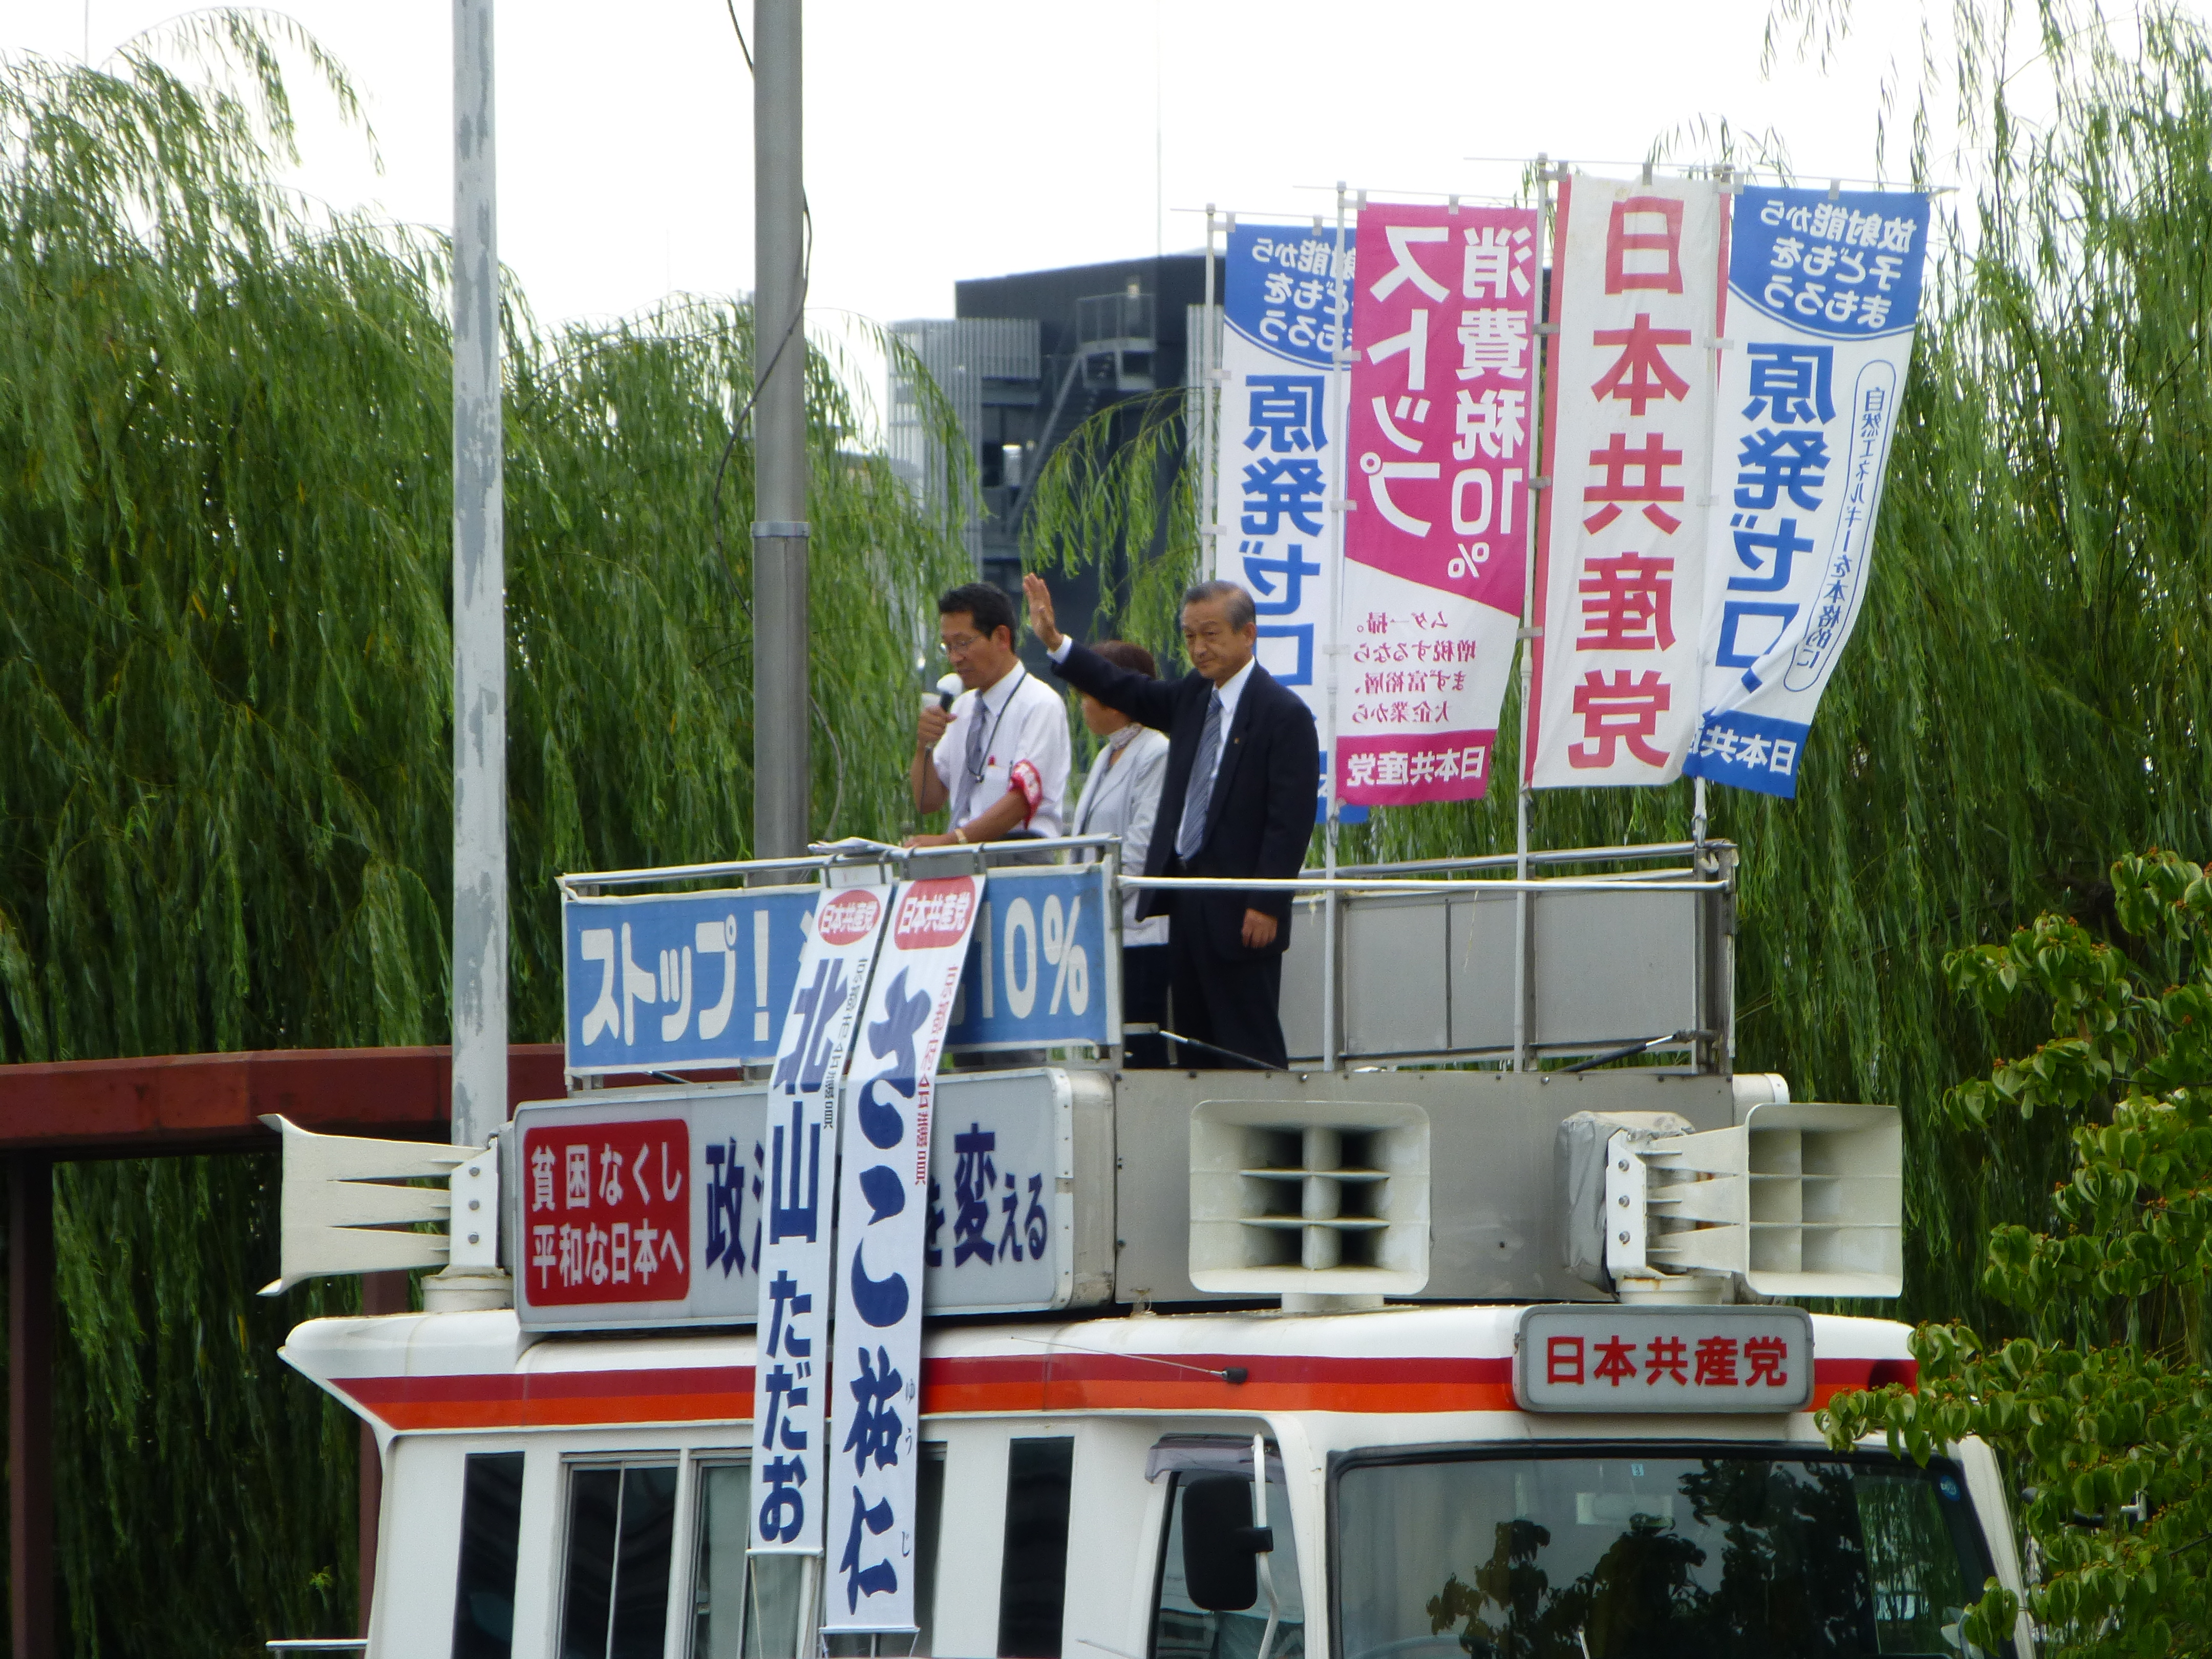
\includegraphics[scale=0.475]
    {figures/jpg/pic11.jpg}
\end{center}
\end{frame}
%-----------------------------------------------------------------------
\section{Strictness}

\begin{frame}[fragile]
\frametitle{Strictness}

\begin{itemize}
\item Imperative languages consist of a sequence of commands.
\item The order in which the commands are executed is specified by
  the language, and the compiler has little freedom to change this
  order.
\item A pure functional language has no commands or side effects,
  only expressions and equations.
\item These can be evaluated in any order without changing the
  result.
\item However, the order of evaluation does affect
  \begin{itemize}
  \item The efficiency of the program, and
  \item whether it terminates at all.
  \end{itemize}
\end{itemize}

\end{frame}

%-----------------------------------------------------------------------
\begin{frame}[fragile]
\frametitle{Defined and undefined values}

\begin{itemize}
\item The aim of a program, of course, is to compute results.
\item Sometimes a program fails to get a result:
  \begin{itemize}
  \item There might be an error: $x/0$ will fail and will not
    produce a number.
  \item The program might go into an infinite loop.
  \end{itemize}
\item A value that the program cannot compute is called $\bot$,
  pronounced \emph{bottom}.
\item The term ``bottom'' comes from domain theory, a branch of
  mathematics which is the foundation of programming language
  theory.  (Yes, there is also $\top$, pronounced \emph{top}.)
\item Any value that cannot be computed is $\bot$ --- the reason
  that it can't be computed (error, loop) is irrelevant.
\end{itemize}

\end{frame}

%-----------------------------------------------------------------------
\begin{frame}[fragile]
\frametitle{Strictness}

An important termination property of a function is its
\emph{strictness}.

\begin{definition}
  A function $f :: a -> b$ is \emph{strict} if and only iff $f \bot
  = \bot$.
\end{definition}

\begin{itemize}
\item If a function is not strict, it is said to be
  \emph{nonstrict}.
\item If a function has several arguments, it may be
  strict/nonstrict in each argument.
\item Strictness is an inherent mathematical property of a
  function, not an implementation detail.
\item In general (with some important exceptions),
  \begin{itemize}
  \item Functions in imperative languages are strict, and
  \item functions in Haskell are nonstrict.
  \end{itemize}
\end{itemize}

\end{frame}

%-----------------------------------------------------------------------
\begin{frame}[fragile]
\frametitle{Bottom in Haskell}

\begin{itemize}
\item Question: what is the type of $\bot$?
\item Answer: it can have any type, because a computation of a
  value of any type could fail to terminate.
\end{itemize}

It's easy to define $\bot$:

\begin{verbatim}
bot :: a
bot = bot
\end{verbatim}

Try it in ghci:

\begin{verbatim}
*Main> :t bot
bot :: a
*Main> bot
^CInterrupted.
*Main> 
\end{verbatim}

\end{frame}

%-----------------------------------------------------------------------
\begin{frame}[fragile]
\frametitle{Example of a strict function}

A strict function:

\begin{verbatim}
f :: Int -> Int
f x = x+1
\end{verbatim}

\begin{verbatim}
*Main> f 3
4
*Main> f bot
^CInterrupted.
*Main> 
\end{verbatim}

\end{frame}

%-----------------------------------------------------------------------
\begin{frame}[fragile]
\frametitle{Example of a nonstrict function}

\begin{verbatim}
g :: Int -> Int -> Int
g x y = x
\end{verbatim}

\begin{verbatim}
*Main> g 3 4       -- Both arguments are defined
3                  --   OK!
*Main> g bot 4     -- First argument is bottom
^CInterrupted.     --   bottom!  g is strict in x
*Main> g 3 bot     -- Second argument is bottom
3                  --   OK!  g is nonstrict in y
*Main> 
\end{verbatim}

\end{frame}

%-----------------------------------------------------------------------
\begin{frame}[fragile]
\frametitle{Partially defined data structures}

\begin{itemize}
\item $[0,1,2,3,4]$ is a fully defined list: all of the list
  structure is defined, and each element is defined.
\item In contrast, $[0,bot,2,bot,4]$ is partially defined:
  \begin{itemize}
  \item All of its list structure is defined, but two of its
    elements are not.
  \end{itemize}
\end{itemize}

\begin{verbatim}
*Main> length [0,1,2,3,4]
5
*Main> [0,1,2,3,4] !! 3
3
*Main> length [0,bot,2,bot,4]
5
*Main> [0,bot,2,bot,4] !! 3
^CInterrupted.
*Main> [0,bot,2,bot,4] !! 4
4
\end{verbatim}

$length$ is nonstrict in the elements of its argument.

\end{frame}

%-----------------------------------------------------------------------
\begin{frame}[fragile]
\frametitle{List with partially defined structure}

\begin{itemize}
\item The list $xs$ has its list structure defined for four
  elements, but
  \begin{itemize}
  \item The value of its second element is undefined, and
  \item The list structure after the fifth element is undefined.
  \end{itemize}
\end{itemize}
{\small
\begin{verbatim}
xs = 0 : 1 : bot : 3 : 4 : bot
xs' = 0 : 1 : bot : 3 : 4 : bot:[]
\end{verbatim}


\begin{verbatim}
Prelude> length xs
^CInterrupted.
Prelude> length xs'
6
Prelude> length (take 4 xs)
4
\end{verbatim}
}
\end{frame}

%-----------------------------------------------------------------------
\begin{frame}[fragile]
\frametitle{Lazy evaluation}

\begin{itemize}
\item Haskell has \emph{nonstrict semantics}.
\item It's often described as a ``pure nonstrict strongly-typed
  functional language''
\item The implementation mechanism used by most Haskell compilers
  to achieve nonstrictness is \emph{lazy evaluation}.
\item The idea behind lazy evaluation:
  \begin{itemize}
  \item The compiler generates object code that evaluates
    expressions \emph{only as they are actually needed}.
  \item If the program actually requires a value, that value is
    computed, and if it is $\bot$ then the program produces $\bot$.
  \item If the program defines a value (in an equation, for
    example) but doesn't actually require it, that value is never
    computed.
  \end{itemize}
\end{itemize}

\end{frame}

%-----------------------------------------------------------------------
\begin{frame}[fragile]
\frametitle{Benefits of nonstrictness (or laziness)}

\begin{itemize}
\item Nonstrictness is pervasive --- it affects all corners of the
  language --- but much of the time you don't need to think about
  it explicitly.
\item But nonstrictness makes possible a variety of useful
  programming techniques, including
  \begin{itemize}
  \item It simplifies formal reasoning, and is useful for proving
    properties of programs.
  \item It allows you to describe a computation more simply, by
    writing equations to define all the values you might need.  As
    long as the values that are actually required are not bottom,
    the program will terminate.
  \item It improves modularity by supporting the ``generate and
    test'' and ``producer and consumer'' paradigms.
  \item It makes possible infinite data structures and data recursion.
  \end{itemize}
\end{itemize}

\end{frame}

%-----------------------------------------------------------------------
\section{Data recursion}

\begin{frame}[fragile]
\frametitle{Data recursion}

\begin{itemize}
\item We've seen recursive functions, where the definition of a
  function $f$ involves calling $f$.
\item We can also define data structures recursively, without
  defining any functions at all.
\item This is an important programming technique in Haskell, with
  many practical applications.
\item It makes essential use of lazy evaluation: data recursion
  won't work in a strict language (although you can simulate it
  with some messy extra work).
\end{itemize}

\end{frame}

%-----------------------------------------------------------------------
\begin{frame}[fragile]
\frametitle{repeat}

The function $repeat$ takes a value and builds an infinite list
containing that value again and again.

\begin{verbatim}
repeat :: a -> [a]
\end{verbatim}

\begin{verbatim}
repeat 3 -- > [3, 3, 3, 3, 3, ...]
\end{verbatim}

Try it yourself: in ghci, just enter {\tt repeat 3}.

\vspace{1em}

If you ever get tired of the output, type Control-C.

\end{frame}

%-----------------------------------------------------------------------
\begin{frame}[fragile]
\frametitle{The implementation of repeat}

\begin{verbatim}
repeat x = xs
  where xs = x : xs
\end{verbatim}

\begin{itemize}
\item The value returned is $xs$.
\item $xs$ is defined to be a cons cell
  \begin{itemize}
  \item Its head field is $x$
  \item Its tail field is a pointer to (the address of) $xs$
  \item Thus the tail of the cell points to the cell.
  \end{itemize}
\item This is a circular data structure.
\item $repeat\; x$ takes up just one cons box (typically two words)
  of memory!
\end{itemize}

\end{frame}

%-----------------------------------------------------------------------
\begin{frame}[fragile]
\frametitle{The semantics of repeat}

\begin{itemize}
\item For any value $x$, the expression $repeat x$ is an infinite
  list of $x$s.
\item In the mathematical semantics of Haskell, this \emph{really
    is an infinite data structure}.
\item $length\, (repeat\; x)$ goes into an infinite loop.
\item You can traverse an infinite data structure.
\item After a finite amount of time, you will have traversed only a
  finite \emph{portion} of the infinite structure.
\item Thus the ``visible'' or ``observed'' part of any data
  structure is always finite, regardless of whether the data
  structure itself is finite or infinite.
\end{itemize}

\end{frame}

%-----------------------------------------------------------------------
\subsection{Fibonacci numbers}

\begin{frame}[fragile]
\frametitle{Fibonacci numbers}

A famous series described by Fibonacci in 1202.

The series is defined using recurrence equations:
$\begin{array}{rcl}
F_{0} &=& 0 \\
F_{1} &=& 1 \\
F_{n} &=& F_{n-2} + F_{n-1}
\end{array}$

\vspace{1em}

Calculating some Fibonacci numbers$\ldots$

\vspace{1em}

$\begin{array}{l}
F_2 = F_0 + F_1 = 0 + 1 = 1 \\
F_3 = F_1 + F_2 = 1 + 1 = 2 \\
F_4 = F_2 + F_3 = 1 + 2 = 3 \\
F_5 = F_3 + F_4 = 2 + 3 = 5 \\
F_6 = F_4 + F_5 = 3 + 5 = 8 \\
F_7 = F_5 + F_6 = 5 + 8 = 13 \\
F_8 = F_6 + F_7 = 8 + 13 = 21 \\
\end{array}$

\end{frame}

%-----------------------------------------------------------------------
\begin{frame}[fragile]
\frametitle{zipWith}

\begin{itemize}
\item A useful helper function is $zipWith$.
\item Motivation$\ldots$ Suppose we have $f :: a->b$, and $xs ::
  [a]$.  Then we can map $f$ over $xs$ with the application $map\, f\,
  xs :: [b]$.
\item But what if we have a function $g :: a -> b -> c$, and we
  want to ``map'' $g$ over the corresponding elements of \emph{two}
  lists, $xs :: [a]$ and $ys :: [b]$?
\item It would be nice to write $map \,g\, (zip\, xs\, ys)$ but this gives
  a type error.  \emph{Why?  what is the error?}
\item Solution: use $zipWith$, a generalisation of $map$ to handle
  functions with two arguments.
\end{itemize}

\begin{verbatim}
zipWith :: (a->b->c) -> [a] -> [b] -> [c]
\end{verbatim}

\begin{verbatim}
zipWith g xs ys :: [c]
\end{verbatim}

\end{frame}

%-----------------------------------------------------------------------
\begin{frame}[fragile]
\frametitle{Infinite list of Fibonacci numbers}

\begin{verbatim}
fibs = xs
  where xs = 0 : 1 : zipWith (+) xs (tail xs)
\end{verbatim}

\begin{verbatim}
*Main> take 20 fibs
[0,1,1,2,3,5,8,13,21,34,55,89,144,233,377,610,
 987,1597,2584,4181]
*Main> 
\end{verbatim}

\end{frame}

%-----------------------------------------------------------------------
\begin{frame}[fragile]
\frametitle{It really is an infinite list}

{\footnotesize
\begin{verbatim}
*Main> fibs
[0,1,1,2,3,5,8,13,21,34,55,89,144,233,377,610,987,1597,2584,
4181,6765,10946,17711,28657,46368,75025,121393,196418,317811,
514229,832040,1346269,2178309,3524578,5702887,9227465,14930352,
24157817,39088169,63245986,102334155,165580141,267914296,
433494437,701408733,1134903170,1836311903,2971215073,4807526976,
7778742049,12586269025,20365011074,32951280099,53316291173,
86267571272,139583862445,225851433717,365435296162,591286729879,
956722026041,1548008755920,2504730781961,4052739537881,
6557470319842,10610209857723,17167680177565,27777890035288,
44945570212853,72723460248141,117669030460994,190392490709135,
308061521170129,498454011879264,806515533049393,1304969544928657,
2111485077978050,3416454622906707,5527939700884757,
8944394323791464,14472334024676221,23416728348467685,
37889062373143906,61305790721611591,99194853094755497,
160500643816367088,259695496911122585,420196140727489673,
679891637638612258,1100087778366101931,1779979416004714189,
2880067194370816120,4660046610375530309,7540113804746346429,
12200160415121876738,19740274219868223167,31940434634990099905,
51680708854858323072,83621143489848422977,135301852344706746049,
\end{verbatim}
}

\end{frame}

%-----------------------------------------------------------------------
\subsection{Modularity and infinite data structures}
\begin{frame}[fragile]
\frametitle{Modularity and infinite data structures}

\begin{itemize}
\item Infinite data structures can help you to improve the
  modularity of a program, improving the structure, readability,
  and maintainability.
\item Consider an algorithm that \emph{produces} some intermediate
  data, and later \emph{consumes} it to give the final results.
\item The idea:
  \begin{itemize}
  \item First module: define an infinite data structure containing
    \emph{all} the values you might need.
  \item Second module: define a consumer that merely looks up the
    values it needs from the data structure.  It knows the value it
    needs will be there, because \emph{all possible values} are in
    the infinite structure.
  \end{itemize}
\item Result: we have completely decoupled the producer and the consumer.
\item Contrast this with what you do in an imperative language: you
  mix up the producer code with the consumer code, because the
  producer doesn't know \emph{which} values to produce.
\end{itemize}

\end{frame}

%-----------------------------------------------------------------------
\section{Advice on structuring a program}
\begin{frame}[fragile]
\frametitle{Advice on structuring a program}

\begin{itemize}
\item In block-structured imperative languages, it's common to have
  very long blocks of code with deep nesting.
\item In Haskell, good style is to have a large number of rather
  small top-level definitions.
\item Generally, try to keep each definition short enough so it
  fits entirely on an editor screen, without scrolling.
\item Incorporate unit tests: either beside the definitions, or in
  a separate module.
%\item Unit tests may be inside comments, so you can copy and paste them into a ghci window.
\item You can write helper functions to run big  collections of unit tests automatically, and check that they got
  the right results.
\end{itemize}

\end{frame}

%-----------------------------------------------------------------------
\begin{frame}[fragile]
\frametitle{Developing an interpreter}

\begin{itemize}
\item An interpreter contains several orthogonal pieces:
  \begin{itemize}
  \item Abstract syntax tree, defined as an algebraic data type
  \item A parser
  \item A traversal of the abstract syntax
  \end{itemize}
\item For good modularity, all these pieces should be defined and
  tested separately.
\item It is \emph{not} necessary to develop the parts of the
  program in the order that you think they will be executed.
\item It's best to start in the middle, with the abstract syntax
  tree.
\end{itemize}

\end{frame}

%-----------------------------------------------------------------------
\begin{frame}[fragile]
\frametitle{Incremental development of traversal}

\begin{itemize}
\item The heart of an interpreter is a recursive function that
  \begin{itemize}
  \item Traverses the tree structure denoting the target program, and
  \item performs the computations called for by the program's
    statements.
  \end{itemize}
\item To understand better what your program is doing, you could
  start with an experimental test program:
  \begin{itemize}
  \item Write a sample program in your target language.
  \item Write a Haskell program, using the IO monad, that performs
    the same computation directly (\emph{without} the tree
    traversal).
  \end{itemize}
\end{itemize}

\end{frame}

%-----------------------------------------------------------------------
\section{Real world parsing examples}
\begin{frame}[fragile]
\frametitle{Real world parsing examples}

\begin{itemize}
\item Some parsing examples taken from a real piece of software:
  the Sigma16 Assembler.
\item Some of the details are omitted or simplified.
\item The real parser handles comments, and also has facilities to
  provide meaningful error messages --- those issues are ignored
  here.
\end{itemize}

\end{frame}

%-----------------------------------------------------------------------
\begin{frame}[fragile]
\frametitle{White space characters}

\begin{verbatim}
listWhiteSpaceChars :: String
listWhiteSpaceChars = [' ', '\t', '\r']
\end{verbatim}

\begin{verbatim}
nonWhiteSpaceChar :: Parser Char
nonWhiteSpaceChar =
  do  x <- noneOf ('\n' : ';' : listWhiteSpaceChars)
      return x
\end{verbatim}

\end{frame}

%-----------------------------------------------------------------------
\begin{frame}[fragile]
\frametitle{White space and text}

\begin{verbatim}
skipWhiteSpace :: Parser ()
skipWhiteSpace =
  do  many whiteSpaceChar
      option () comment
      return ()
\end{verbatim}

\begin{verbatim}
nonWhite :: Parser String
nonWhite =
  do  xs <- many nonWhiteSpaceChar
      return xs
\end{verbatim}

\end{frame}

%-----------------------------------------------------------------------
\begin{frame}[fragile]
\frametitle{Splitting a line into fields}

\begin{verbatim}
getFields :: Parser (String,String,String,String)
getFields =
  do  f1 <- nonWhite
      skipWhiteSpace
      f2 <- nonWhite
      skipWhiteSpace
      f3 <- nonWhite
      f4 <- restOfLine
      return (f1,f2,f3,f4)
\end{verbatim}

\end{frame}

%-----------------------------------------------------------------------
\begin{frame}[fragile]
\frametitle{Parsing a register}
{\small
\begin{verbatim}
register :: Parser RegisterSrc
register = try regDecNumber <|> regHexNumber
\end{verbatim}
}
The register number can be a single hexadecimal digit
{\small
\begin{verbatim}
regHexNumber :: Parser RegisterSrc
regHexNumber =
  do  r <- oneOf "rR"
      x <- hexDigit
      return (RegHex x)
\end{verbatim}
}
Alternatively, the register number can be a string of decimal
digits.
{\small
\begin{verbatim}
regDecNumber :: Parser RegisterSrc
regDecNumber =
  do  r <- oneOf "rR"
      x <- digit
      xs <- many digit
      return (RegDec (x:xs))
\end{verbatim}
}
\end{frame}

%-----------------------------------------------------------------------
\begin{frame}[fragile]
\frametitle{RRR format operands}

\begin{verbatim}
"R3,R4,R5"
"R0,Rc,R9"
\end{verbatim}

\begin{verbatim}
rrrField :: Parser RRR_operand_src
rrrField =
  do  r1 <- register
      char ','
      r2 <- register
      char ','
      r3 <- register
      eof
      return (RRR_syntax_ok r1 r2 r3)
\end{verbatim}

\end{frame}

%-----------------------------------------------------------------------
\begin{frame}[fragile]
\frametitle{RX format operands}

\begin{verbatim}
"R2,variable[R0]"
"R1,234[Ra]"
\end{verbatim}

\begin{verbatim}
rxField :: Parser RX_operand_src
rxField =
  do  r <- register
      char ','
      a <- dispBase
      return (RX_syntax_ok r a)
\end{verbatim}

\end{frame}

%-----------------------------------------------------------------------
\begin{frame}[fragile]
\frametitle{Displacement field}
     
\begin{verbatim}
dispBase :: Parser (Val16, RegisterSrc)
dispBase =
  do  disp <- val16
      char '['
      r <- register
      char ']'
      return (disp,r)
\end{verbatim}

\end{frame}

%-----------------------------------------------------------------------
\section{Unassessed exercises}

\begin{frame}[fragile]
\frametitle{Unassessed exercises}

\begin{enumerate}

\item Work out the value of $map\, abs\, [0, -4, 7, -2, 9]$.

\item Work out the value of $foldl\, (+)\, 100\, [2,7,3]$.

\item Work out the value of $foldr\, (+)\, 100\, [2,7,3]$.

\item Work out the value of $foldl\, (-)\, 100\, [2,7,3]$.

\item Work out the value of $foldr\, (-)\, 100\, [2,7,3]$.

\item Write a parser $simpleVar$ that accepts a variable name
  consisting only of letters and underscores (the {\tt \_ } character).
  The variable name must contain at least one character, and it may
  begin with either a letter or underscore.

\item Write a parser $betterVar$ that accepts a better form of
  variable name, which may contain letters, digits, underscores
  (the {\tt \_}character), primes (the {\tt '} character).
  The variable name must begin with a letter.  Only one prime is
  allowed in a name, and if a prime appears, it must be the last
  character in the name.
\end{enumerate}

\end{frame}

\end{document}
